\section{Casi d'Uso}
		\subsection{Attori}			
        I casi d'uso definiscono interazioni tra il sistema e gli attori esterni. L'elenco di questi ultimi e l'analisi delle relazioni in funzione dei diversi scopi che questi attori perseguono è fondamentale per una corretta descrizione dei casi d'uso.
        Riportiamo due attori:
        \begin{itemize}
            \item Utente generico
            \item Grafana
        \end{itemize}


		\subsection{Tracciamento Casi d'Uso}
        Al fine di classificare e rendere leggibili i casi d'uso abbiamo deciso di utilizzare una codifica per descriverli. Ad ogni caso d'uso verrà quindi associata una stringa univoca strutturata nel seguente modo: UCX.Y.Z  dove X,Y,Z sono dei numeri progressivi per indicare specificità all'interno dei casi d'uso.

		\subsection{Attore primario: Utente generico}
		Si riferiscono a tutt quei casi d'uso che hanno come attore primario l'utente e come attore secondario Grafana o il nostro sistema. Descrivono tutte le interazioni possibili compiute direttamente dall'utente.
		
		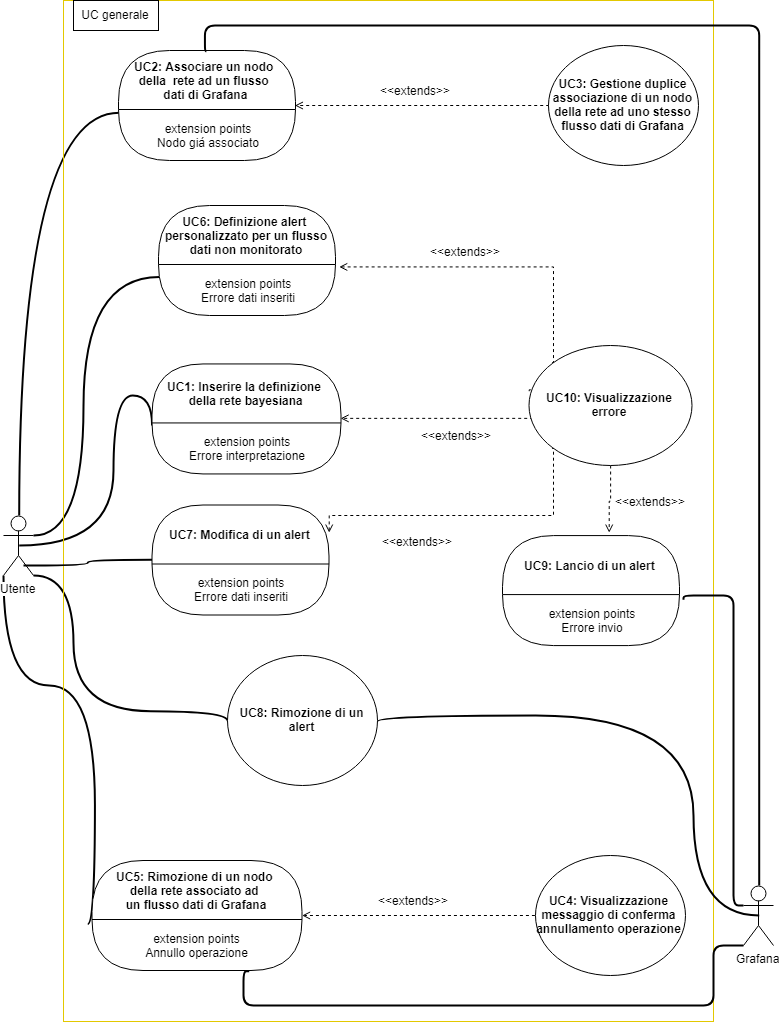
\includegraphics[width=\textwidth]{UC.png}
		
				\subsubsection{UC1: Inserimento definizione rete bayesiana}
                    \textbf{Precondizione:} l’utente deve trovarsi nell’interfaccia principale e deve possedere una definizione di rete bayesiana che vuole inserire.
                    \newline
                    \textbf{Postcondizione:} viene inserita nell’applicativo la definizione di rete.
                    \newline
                    \textbf{Attore primario:} Utente.
                    \newline
                    \textbf{Contestualizzazione / Scenario principale:} l’utente carica la definizione della rete bayesiana.
                    \newline
                    \textbf{Estensioni:} \begin{enumerate}
                            \item Problema con l’interpretazione della rete bayesiana \textbf{UC10}
                        \end{enumerate}
                        
                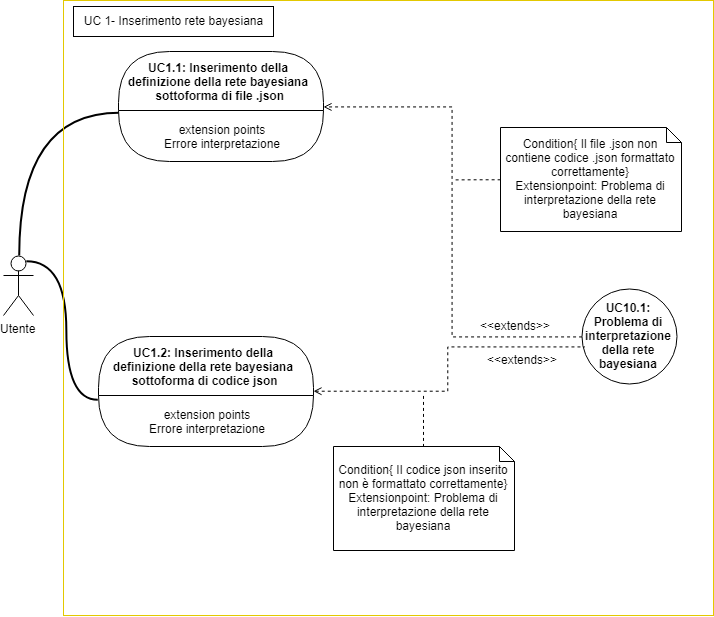
\includegraphics[width=\textwidth]{UC1.png}
                        
                \subsubsection{UC1.1: Inserimento definizione della rete bayesiana sotto forma di file .json}
                    \textbf{Precondizione:}  l’utente deve trovarsi nell’interfaccia principale e possedere un file .json contenente una definizione di rete bayesiana che vuole inserire.
                    \newline
                    \textbf{Postcondizione:} viene inserita nell’applicativo la definizione di rete presente nel file .json.
                    \newline
                    \textbf{Attore primario:} Utente.
                    \newline
                    \textbf{Contestualizzazione / Scenario principale:} \begin{enumerate}
                        \item L’utente preme il pulsante per l’upload del file .json contenente la definizione di rete
                        \item l’utente sceglie il file
                        \item Upload del file
                        \item La rete viene caricata
                    \end{enumerate}
                    
                    \textbf{Estensioni:} \begin{enumerate}
                            \item C’è stato un problema con l’interpretazione della rete bayesiana \textbf{UC10.1}
                        \end{enumerate}
                        
                \subsubsection{UC1.2: Inserimento definizione rete bayesiana sotto forma di codice json}
                    \textbf{Precondizione:}  l’utente deve trovarsi nell’interfaccia principale e possedere codice json di una definizione di rete bayesiana che vuole inserire.
                    \newline
                    \textbf{Postcondizione:} viene inserita nell’applicativo la definizione di rete descritta dal codice json.
                    \newline
                    \textbf{Attore primario:} Utente.
                    \newline
                    \textbf{Contestualizzazione / Scenario principale:} \begin{enumerate}
                        \item l’utente incolla il codice json nel text area dedicata
                        \item l’utente preme il pulsante “Insert Bayesian Network”
                    \end{enumerate}
                    
                    \textbf{Estensioni:} \begin{enumerate}
                            \item C’è stato un problema con l’interpretazione della rete bayesiana \textbf{UC10.1}
                        \end{enumerate}
                        
                \subsubsection{UC2: Associazione un nodo della rete ad un flusso dati di Grafana}
                    \textbf{Precondizione:}   L’utente deve trovarsi nella schermata di impostazioni della rete bayesiana e deve essere presente la definizione della rete bayesiana.
                    \newline
                    \textbf{Postcondizione:} Il nodo delle rete è associato ad un flusso dati.
                    \newline
                    \textbf{Attore primario:} Utente.
                    \newline
                    \textbf{Attore secondario:} Grafana.
                    \newline
                    \textbf{Contestualizzazione / Scenario principale:} \begin{enumerate}
                        \item L’utente seleziona un flusso di monitoraggio
                        \item Seleziona la funzione “associa”
                        \item Sceglie la rete bayesiana di interesse da un elenco (se c’è nè più di una)
                        \item Seleziona il nodo della rete
                        \item Viene visualizzato un messaggio di conferma (“associazione riuscita”)
                    \end{enumerate}
                    
                    \textbf{Estensioni:} \begin{enumerate}
                            \item Gestione duplice associazione di un nodo della rete ad uno stesso flusso dati di Grafana \textbf{UC3}
                        \end{enumerate}
                
                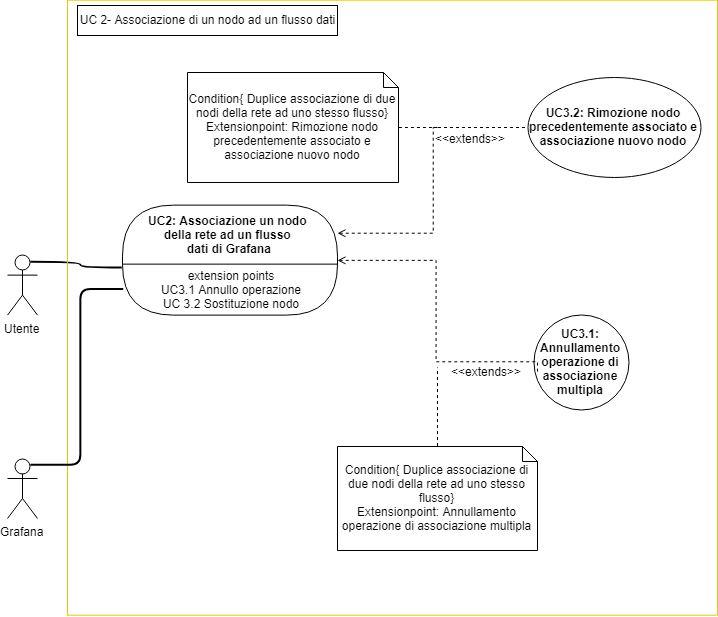
\includegraphics[width=\textwidth]{UC2.png}
                
                \subsubsection{UC3: Gestione duplice associazione di due nodi della rete ad uno stesso flusso dati di Grafana}
                    \textbf{Descrizione:} il sistema avvisa l’utente che é in corso una duplice associazione di due nodi della stessa rete allo stesso flusso di monitoraggio.
                    \newline
                    \textbf{Precondizione:} l’utente ha giá associato ad un nodo della rete il flusso di interesse.
                    \newline
                    \textbf{Postcondizione:}  La rete bayesiana possiede un solo nodo associato al flusso di monitoraggio di interesse.
                    \newline
                    \textbf{Attore primario:} Utente.
                    \newline
                    \textbf{Contestualizzazione / Scenario principale:} \begin{enumerate}
                        \item Viene visualizzato un messaggio di allerta (“Tentativo duplice associazione”)
                        \item All’utente vengono proposte due scelte:
                                \begin{enumerate}
                                    \item Annullamento operazione associazione multipla \textbf{UC3.1}
                                    \item Rimozione nodo precedentemente associato e associazione nuovo nodo \textbf{UC3.2}
                                \end{enumerate}
                    \end{enumerate}
                
                \subsubsection{UC3.1: Annullamento operazione associazione multipla}
                    \textbf{Descrizione:}  l’utente richiede l’annullamento dell’operazione.
                    \newline
                    \textbf{Precondizione:} Si e’ verificata un tentativo di associazione multipla e l’utente ha deciso di annullare l’operazione.
                    \newline
                    \textbf{Postcondizione:}  Il sistema annulla l’operazione.
                    \newline
                    \textbf{Attore primario:} Utente.
                    \newline
                    \textbf{Contestualizzazione / Scenario principale:} \begin{enumerate}
                        \item Visualizzazione messaggio di conferma annullamento operazione \textbf{UC4}
                    \end{enumerate}
                
                \subsubsection{UC3.2: Rimozione nodo precedentemente associato e associazione nuovo nodo}
                    \textbf{Descrizione:} l’utente richiede la sostituzione del nodo correntemente associato con un nuovo nodo a sua scelta.
                    \newline
                    \textbf{Precondizione:}  Si e’ verificata un tentativo di associazione multipla e l’utente ha deciso di rimuovere il nodo precedentemente associato.
                    \newline
                    \textbf{Postcondizione:} Al flusso di monitoraggio verrá associato un nuovo nodo della rete secondo la volontá dell’utente.
                    \newline
                    \textbf{Attore primario:} Utente.
                    \newline
                    \textbf{Contestualizzazione / Scenario principale:} \begin{enumerate}
                        \item Rimozione di un nodo della rete associato ad un flusso \textbf{UC5}
                        \item Associazione un nodo della rete ad un flusso \textbf{UC2}
                    \end{enumerate}
                    
                \subsubsection{UC4: Visualizzazione messaggio di conferma annullamento operazione}
                    \textbf{Descrizione:} il sistema avvisa l’utente che è in corso l’annullamento dell’operazione.
                    \newline
                    \textbf{Precondizione:} l’utente vuole annullare un’operazione.
                    \newline
                    \textbf{Postcondizione:} Il sistema annulla l’operazione.
                    \newline
                    \textbf{Attore primario:} Utente.
                    \newline
                    \textbf{Contestualizzazione / Scenario principale:} \begin{enumerate}
                        \item il sistema presenta all’utente un messaggio di conferma annullamento
                        \item l’utente conferma di voler annullare 
                        \item l’utente viene reindirizzato alla pagina principale
                    \end{enumerate}
                    
                \subsubsection{UC5: Rimozione di un nodo della rete associato ad un flusso dati di Grafana}
                    \textbf{Descrizione:} L'utente vuole rimuovere un'associazione tra un flusso dati monitorato in Grafana e un nodo della rete bayesiana.
                    \newline
                    \textbf{Precondizione:} L’utente deve trovarsi nella schermata di impostazioni della rete bayesiana e un nodo della rete deve essere stato associato al flusso di monitoraggio (postcondizione di \textbf{UC2}).
                    \newline
                    \textbf{Postcondizione:} Viene rimossa l’associazione del nodo di interesse al flusso dati.
                    \newline
                    \textbf{Attore primario:} Utente.
                    \newline
                    \textbf{Attore secondario:} Grafana.
                    \newline
                    \textbf{Contestualizzazione / Scenario principale:} \begin{enumerate}
                            \item L’utente seleziona un flusso di monitoraggio
                            \item Seleziona la funzione “rimuovi associazione” 
                            \item Viene visualizzato un messaggio di conferma (“rimozione riuscita”)
                        \end{enumerate}
                    
                    \textbf{Estensioni:} 
                    \begin{enumerate}
                            \item Visualizzazione messaggio di conferma annullamento operazione \textbf{UC4}
                        \end{enumerate}
                        
                \subsubsection{UC6: Definizione alert personalizzato per un flusso dati non monitorato}
                    \textbf{Descrizione:} l’utente desidera creare un alert associato ad un flusso dati non monitorato su Grafana ed e’ gia’ sulla sezione alert di edit di un panel
                    \newline
                    \textbf{Precondizione:} sono presenti dei flussi dati non monitorati su Grafana.
                    \newline
                    \textbf{Postcondizione:} e’ stato definito un alert personalizzato per il flusso dati.
                    \newline
                    \textbf{Attore primario:} Utente.
                    \newline
                    \textbf{Attore secondario:} Grafana.
                    \newline
                    \textbf{Contestualizzazione / Scenario principale:} \begin{enumerate}
                            \item L’utente preme sul pulsante “create alert”
                            \item L’utente configura l’alert 
                            \item L’utente salva la dashboard
                        \end{enumerate}
                    
                    \textbf{Estensioni:} 
                    \begin{enumerate}
                            \item Errore nei dati inseriti per la creazione dell'alert \textbf{UC10.3}
                        \end{enumerate}
                
                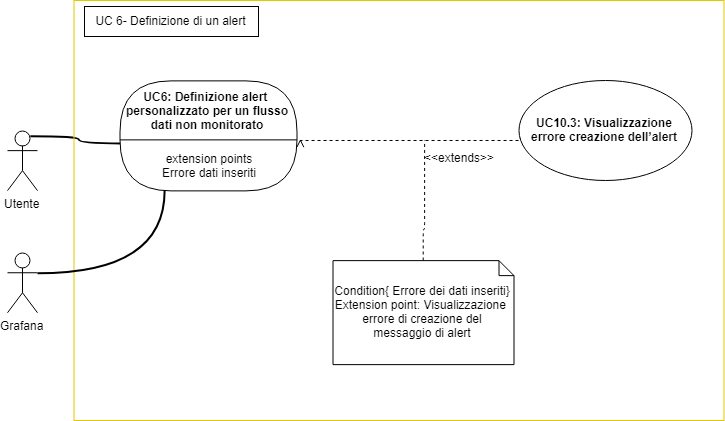
\includegraphics[width=\textwidth]{UC6.png}
                
                \subsubsection{UC7: Modifica di un alert}
                    \textbf{Descrizione:} l’utente desidera modificare un alert associato ad un flusso dati non monitorato su Grafana ed e’ gia’ sulla sezione alert di edit di un panel.
                    \newline
                    \textbf{Precondizione:} sono presenti dei flussi dati non monitorati su Grafana e esiste un alert a loro associato.
                    \newline
                    \textbf{Postcondizione:} e’ stato modificato un alert personalizzato per il flusso dati.
                    \newline
                    \textbf{Attore primario:} Utente.
                    \newline
                    \textbf{Attore secondario:} Grafana.
                    \newline
                    \textbf{Contestualizzazione / Scenario principale:} \begin{enumerate}
                            \item L’utente configura l’alert 
                            \item L’utente salva la dashboard
                        \end{enumerate}
                    
                    \textbf{Estensioni:} 
                    \begin{enumerate}
                            \item Errore nei dati inseriti per la creazione dell'alert \textbf{UC10.3}
                        \end{enumerate}
                        
                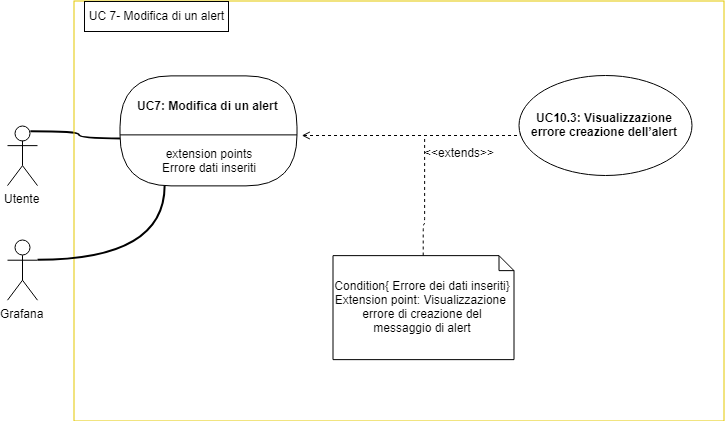
\includegraphics[width=\textwidth]{UC7.png}
                        
                \subsubsection{UC8: Rimozione di un alert}
                    \textbf{Descrizione:}  l’utente desidera eliminare un alert associato ad un flusso dati non monitorato su Grafana.
                    \newline
                    \textbf{Precondizione:} sono presenti dei flussi dati non monitorati su Grafana e esiste un alert a loro associato.
                    \newline
                    \textbf{Postcondizione:} e’ stato rimosso un alert personalizzato per il flusso dati.
                    \newline
                    \textbf{Attore primario:} Utente.
                    \newline
                    \textbf{Attore secondario:} Grafana.
                    \newline
                    \textbf{Contestualizzazione / Scenario principale:} \begin{enumerate}
                            \item L’utente preme sul pulsante “delete”
                            \item L’utente salva la dashboard
                        \end{enumerate}
				
		\subsection{Attore primario: Granafa}	
		
		        \subsubsection{UC9: Lancio di un alert}
                    \textbf{Descrizione:} Grafana ha rilevato che una delle condizioni dell'alert sono state violate e avviene quindi il "lancio" dell'alert stesso.
                    \newline
                    \textbf{Precondizione:} Il flusso di monitoraggio (G) di interesse ha un alert ed è associato ad un nodo di una rete bayesiana.
                    \newline
                    \textbf{Postcondizione:} Vengonono interpretati i dati per il ricalcolo delle probabilità con il contributo di “jsbayes”.
                    \newline
                    \textbf{Attore primario:} Grafana.
                    \newline
                    \textbf{Contestualizzazione / Scenario principale:} \begin{enumerate}
                            \item Grafana rileva che un flusso di monitoraggio (G) non rispetta le condizioni di uno dei suoi alert
                            \item Grafana invia il messaggio di alert al sistema (noi siamo il sistema a cui invia i dati di alert)
                            \item I dati vengono gestiti e con l’ausilio della libreria jsbayes vengono ricalcolate le probabilità dei nodi non monitorati
                        \end{enumerate}
                    
                    \textbf{Estensioni:} 
                    \begin{enumerate}
                            \item Viene visualizzato un errore di invio messaggio di alert \textbf{UC6.2}
                        \end{enumerate}
                        
                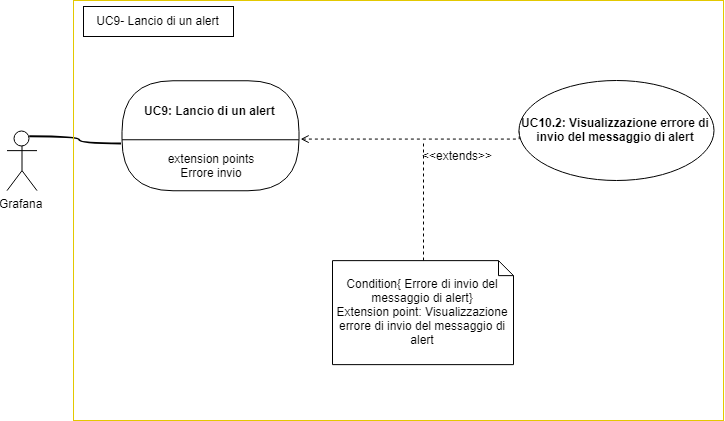
\includegraphics[width=\textwidth]{UC9.png}
                        
                \subsubsection{UC10: Visualizzazione errore}
                    \textbf{Descrizione:}  il sistema avvisa l’utente che c’é stato un errore.
                    \newline
                    \textbf{Precondizione:} sono avvenute delle operazioni non consentite.
                    \newline
                    \textbf{Postcondizione:} l’utente e’ consapevole di trovarsi in uno stato di errore.
                    \newline
                    \textbf{Attore primario:} Grafana.
                    \newline
                    \textbf{Attore secondario:} Utente.
                    \newline
                    \textbf{Contestualizzazione / Scenario principale:} \begin{enumerate}
                            \item il sistema avvisa l’utente tramite un messaggio di errore
                            \item l’utente viene rimandato alla pagina principale
                        \end{enumerate}
                        
                \subsubsection{UC10.1: Visualizzazione errore interpretazione rete bayesiana}
                    \textbf{Descrizione:}  il sistema avvisa l’utente che la rete bayesiana non e’ stata interpretata correttamente e non puó essere inserita.
                    \newline
                    \textbf{Precondizione:} l’utente tenta di inserire una rete bayesiana non formattata correttamente.
                    \newline
                    \textbf{Postcondizione:} l’utente e’ consapevole di aver inserito una rete bayesiana non formattata correttamente.
                    \newline
                    \textbf{Attore primario:} Grafana.
                    \newline
                    \textbf{Attore secondario:} Utente.
                    \newline
                    \textbf{Contestualizzazione / Scenario principale:} \begin{enumerate}
                            \item il sistema avvisa l’utente tramite un messaggio di errore
                            \item l’utente viene rimandato all’interfaccia di upload
                        \end{enumerate}
                
                \subsubsection{UC10.2: Visualizzazione errore invio del messaggio di alert}
                    \textbf{Descrizione:} il sistema avvisa l’utente che e’ avvenuto un errore nell’invio dell’alert.
                    \newline
                    \textbf{Precondizione:} e’ avvenuto un errore nell’invio dell’alert da parte di Grafana.
                    \newline
                    \textbf{Postcondizione:} l’utente e’ consapevole dell’errore nell’invio dell’alert.
                    \newline
                    \textbf{Attore primario:} Grafana.
                    \newline
                    \textbf{Attore secondario:} Utente.
                    \newline
                    \textbf{Contestualizzazione / Scenario principale:} \begin{enumerate}
                            \item il sistema avvisa l’utente tramite un messaggio di errore e tramite l’invio di una mail
                        \end{enumerate}
                        
                \subsubsection{UC10.3: Visualizzazione errore configurazione dell’alert}
                    \textbf{Descrizione:} il sistema avvisa l’utente che e’ avvenuto un errore nella configurazione dell’alert.
                    \newline
                    \textbf{Precondizione:}  e’ avvenuto un errore nell’inserimento dei dati nell’alert da parte dell’utente.
                    \newline
                    \textbf{Postcondizione:} l’utente e’ consapevole dell’errore di creazione dell’alert.
                    \newline
                    \textbf{Attore primario:} Grafana.
                    \newline
                    \textbf{Attore secondario:} Utente.
                    \newline
                    \textbf{Contestualizzazione / Scenario principale:} \begin{enumerate}
                            \item il sistema avvisa l’utente tramite un messaggio di errore
                        \end{enumerate}
\newpage
